\PassOptionsToPackage{table}{xcolor}
\documentclass[presentation,t]{beamer}
%\usetheme{Antibes}
%\usetheme{Boadilla}
\usetheme{default}
\usecolortheme{dolphin}
\useinnertheme{rectangles}
%\useoutertheme{infolines}
%\usepackage{amsmath}
\usepackage{amsthm}
\usepackage{amssymb}
\usepackage{graphicx}
\usepackage{fullpage}
\usepackage{enumerate}
\usepackage{array}
\usepackage{multicol}
%\usepackage{youngtab}
\usepackage{float}

\usepackage[utf8x]{inputenc}
\usepackage{default}
\usepackage{amssymb,amsfonts,amsbsy,amsmath}
%\usepackage{tkz-graph}
\usepackage{amsmath}
\usepackage{graphicx}

\newcommand{\mycirc}[1]
{\textcircled{\raisebox{-.8pt}{#1}}}

\newcommand{\mytwo}[2]
{\raisebox{1.1pt}{\scriptsize #1} \hspace{1pt} \raisebox{-1.1pt}{\scriptsize #2}}


%% Some useful operatorname declarations for nice texing.
\newcommand{\Aut}{\operatorname{Aut}}
\newcommand{\Inn}{\operatorname{Inn}}
\newcommand{\Ker}{\operatorname{Ker}}
\newcommand{\Stab}{\operatorname{Stab}}
\newcommand{\orb}[1]{\mathcal{O}_#1}
\newcommand{\lcm}{\operatorname{lcm}}
\newcommand{\U}{\operatorname U}
\newcommand{\cl}{\operatorname {cl}}

%% Stuff from King's .tex files
\newcommand{\untab}{\noindent \!\!\!\!\!\!\!\!\!}
\newcommand{\lra}{\longrightarrow}
\newcommand{\mb}[1]{\mathbf{#1}}
\newcommand{\gap}{\vspace{0.1in}}
\DeclareMathOperator{\grad}{grad}
\DeclareMathOperator{\curl}{curl}
\DeclareMathOperator{\GL}{GL}
\newcommand{\myline}
{\vspace{.2in}
  \begin{center}
    \rule{5in}{.7pt}
  \end{center}
  \vspace{.2in}}

\usepackage{parskip}

\setlength{\parindent}{2ex}
\setlength{\parskip}{2ex plus 1ex minus 1ex}


%%% Good old "not sure if equal"
\newcommand{\qe}{\stackrel{?}{=}}

%% Some quickies for the big groups
\newcommand{\Q}{\mathbb Q}
\newcommand{\F}{\mathbb F}
\newcommand{\Qp}{\mathbb Q^+}
\newcommand{\Qn}{\mathbb Q^-}
\newcommand{\Qs}{\mathbb Q^*}
\newcommand{\R}{\mathbb R}
\newcommand{\Rp}{\mathbb R^+}
\newcommand{\Rn}{\mathbb R^-}
\newcommand{\Rs}{\mathbb R^*}
\newcommand{\Z}{\mathbb Z}
%\newcommand{\N}{\mathbb N}
%\newcommand{\C}{\mathbb C}

\newcommand{\Af}{\mathbb A}
\newcommand{\PP}{\mathbb P}

\newcommand{\GF}{\mathbb GF}

\newcommand{\gl}{\mathfrak g}
\newcommand{\bl}{\mathfrak b}
\newcommand{\tl}{\mathfrak t}
\newcommand{\pl}{\mathfrak p}
\newcommand{\nl}{\mathfrak n}

\DeclareMathOperator{\sh}{sh}

\newcommand{\Orb}{\mathcal O}
\newcommand{\Var}{\mathcal V}

\newcommand{\Irr}{\operatorname{Irr}}

\newcommand{\Brak}{[\cdot,\cdot]}

\newcommand{\NWN}{\nl \cap {^w\nl}}
\newcommand{\closeGNWN}{\overline{G \cdot (\NWN)}}

\newcommand{\N}{\mathbb N}
\newcommand{\C}{\mathbb C}

\newcommand{\GLn}{GL_n(\C)}
\newcommand{\gln}{\mathfrak {gl}_n}

\newcommand{\rank}{\operatorname{Rank}}

\newcommand{\bracket}{[\cdot, \cdot]}

\newcommand{\LRGfxSymArrowTwo}[2]{%
  \raisebox{1.3cm}{ \centering \parbox{.6cm}{ \centering%
    {\scriptsize $#1$}\\[-.23cm]$\longrightarrow$\\[-.3cm]%
    $\longleftarrow$\\[-.23cm] {\scriptsize $#2$}%
  } }%
}

% \newcommand{\LRGfxSymArrowTwo}[2]{
%   \raisebox{1.3cm}{
%     \begin{tabular}{c}
%       \centering%
%       {\scriptsize $#1$}\\[-.23cm]
%       $\longrightarrow$\\[-.3cm]%
%       $\longleftarrow$\\[-.23cm]
%       {\scriptsize $#2$}%
%     \end{tabular}
%   }
% }

\newcommand{\LRGfxSymArrow}[1]{
  \LRGfxSymArrowTwo{#1}{#1}
}
%% Good old "not sure if equal"
\newcommand{\qe}{\stackrel{?}{=}}

\makeatletter
\DeclareRobustCommand{\em}{%
  \@nomath\em \if b\expandafter\@car\f@series\@nil
  \normalfont \else \bfseries \fi}
\makeatother
\renewcommand<>{\emph}[1]{{\em #1}}

%% Some quickies for the big groups
\newcommand{\Q}{\mathbb Q}
\newcommand{\F}{\mathbb F}
\newcommand{\Qp}{\mathbb Q^+}
\newcommand{\Qn}{\mathbb Q^-}
\newcommand{\Qs}{\mathbb Q^*}
\newcommand{\R}{\mathbb R}
\newcommand{\Rp}{\mathbb R^+}
\newcommand{\Rn}{\mathbb R^-}
\newcommand{\Rs}{\mathbb R^*}
\newcommand{\Z}{\mathbb Z}
%\newcommand{\N}{\mathbb N}
%\newcommand{\C}{\mathbb C}

\newcommand{\Af}{\mathbb A}
\newcommand{\PP}{\mathbb P}

\newcommand{\GF}{\mathbb GF}

\newcommand{\gl}{\mathfrak g}
\newcommand{\bl}{\mathfrak b}
\newcommand{\tl}{\mathfrak t}
\newcommand{\pl}{\mathfrak p}
\newcommand{\nl}{\mathfrak n}

\DeclareMathOperator{\sh}{sh}

\newcommand{\Orb}{\mathcal O}
\newcommand{\Var}{\mathcal V}

\newcommand{\Irr}{\operatorname{Irr}}

\newcommand{\Brak}{[\cdot,\cdot]}

\newcommand{\NWN}{\nl \cap {^w\nl}}
\newcommand{\closeGNWN}{\overline{G \cdot (\NWN)}}

\newcommand{\N}{\mathbb N}
\newcommand{\C}{\mathbb C}

\newcommand{\GLn}{GL_n(\C)}
\newcommand{\gln}{\mathfrak {gl}_n}

\newcommand{\rank}{\operatorname{Rank}}


\newcommand{\loopinsert}{E_1}
\newcommand{\edgedouble}{E_2}
\newcommand{\cutedgedouble}{E_3}
\newcommand{\pairinsert}{E_4}
\newcommand{\plantri}{\textit{plantri} }
\newcommand{\nauty}{\textit{nauty} }
\newcommand{\saucy}{\textit{saucy} }
\newcommand{\valgrind}{\textit{valgrind} }


\usepackage{overpic}
%\usepackage{svg}
\usepackage{graphicx}
%\usepackage{mathrsfs}
%\usepackage{setspace}
%\usepackage{showkeys}
\usepackage{amsmath}
\usepackage{hyperref}
\usepackage{tikz}
\usepackage{pgfplots}
\usepackage{pgfplotstable}
\usepackage{array}
\pgfplotsset{compat=newest}
\usetikzlibrary{positioning,arrows,knots,calc,decorations.markings}
\usepgfplotslibrary{colorbrewer}

\definecolor{beamerblue}{RGB}{234,233,243}
\definecolor{beamerviolet}{RGB}{47,23,132}
\definecolor{beamerliteviolet}{RGB}{137,127,207}

\tikzset{onslide/.code args={<#1>#2}{%
  \only<#1>{\pgfkeysalso{#2}} % \pgfkeysalso doesn't change the path
}}
\tikzset{temporal/.code args={<#1>#2#3#4}{%
  \temporal<#1>{\pgfkeysalso{#2}}{\pgfkeysalso{#3}}{\pgfkeysalso{#4}} % \pgfkeysalso doesn't change the path
}}

\tikzset{
  invisible/.style={opacity=0},
  visible on/.style={alt={#1{}{invisible}}},
  alt/.code args={<#1>#2#3}{%
    \alt<#1>{\pgfkeysalso{#2}}{\pgfkeysalso{#3}} % \pgfkeysalso doesn't change the path
  },
}

\pgfplotsset{
  /pgfplots/bar cycle list/.style={/pgfplots/cycle list={%
      {RdBu-10-1!50!black,fill=RdBu-10-1!80!white,mark=none},%
      {RdBu-10-2!50!black,fill=RdBu-10-2!80!white,mark=none},%
      {RdBu-10-3!50!black,fill=RdBu-10-3!80!white,mark=none},%
      {RdBu-10-4!50!black,fill=RdBu-10-4!80!white,mark=none},%
      {RdBu-10-5!50!black,fill=RdBu-10-5!80!white,mark=none},%
      {RdBu-10-6!50!black,fill=RdBu-10-6!80!white,mark=none},%
      {RdBu-10-7!50!black,fill=RdBu-10-7!80!white,mark=none},%
      {RdBu-10-8!50!black,fill=RdBu-10-8!80!white,mark=none},%
      {RdBu-10-9!50!black,fill=RdBu-10-9!80!white,mark=none},%
      {RdBu-10-10!50!black,fill=RdBu-10-10!80!white,mark=none},%
    }
  },
}

% \pgfplotsset{
%   /pgfplots/bar cycle list/.style={/pgfplots/cycle list={%
%       {red!80!black,fill=red!30!white,mark=none},%
%       {orange!80!black,fill=orange!30!white,mark=none},%
%       {yellow!80!black,fill=yellow!30!white,mark=none},%
%       {lime!80!black,fill=lime!30!white,mark=none},%
%       {green!80!black,fill=green!30!white,mark=none},%
%       {teal!80!black,fill=teal!30!white,mark=none},%
%       {cyan!80!black,fill=cyan!30!white,mark=none},%
%       {blue!80!black,fill=blue!30!white,mark=none},%
%       {violet!80!black,fill=violet!30!white,mark=none},%
%       {purple!80!black,fill=purple!30!white,mark=none},%
%     }
%   },
% }


\newcommand{\Uhyp}{\mathcal U} \newcommand{\Vhyp}{\mathcal V}
\newcommand{\Rhyp}{\mathcal R}


\title{Random Knot Diagrams}
\author[Cantarella, Chapman, Mastin]{Harrison Chapman (UGA - Graduate
  student)\\joint w/ Jason Cantarella (UGA), Matt Mastin (Wake Forest)}
\date[AMS Sectionals 2015]{AMS Western Spring Sectionals 2015 (UNLV) -- April 18, 2015}

%\allowdisplaybreaks
%\usepackage[bookmarks,bookmarksopen,bookmarksdepth=4]{hyperref}

\newcommand{\so}[1]{\mathfrak {so}(#1)}

%\newtheorem{theorem}{Theorem}[section]
%\newtheorem{lemma}[theorem]{Lemma}
%\newtheorem{definition}[theorem]{Definition}
\newtheorem{proposition}[theorem]{Proposition}
%\newtheorem{corollary}[theorem]{Corollary}

%\renewcommand*\showkeyslabelformat[1]{\normalfont\tiny\ttfamily(#1)}

\graphicspath{{../../figs/}{figs/}}

\let\oldemptyset\emptyset
\let\emptyset\varnothing

\DeclareMathOperator{\Arm}{Arm}
\DeclareMathOperator{\Pol}{Pol}
\DeclareMathOperator{\UP}{UP}
\DeclareMathOperator{\VP}{VP}
\DeclareMathOperator{\APol}{APol}
\DeclareMathOperator{\Diff}{Diff}
\DeclareMathOperator{\Sympl}{Sympl}
\DeclareMathOperator{\ev}{ev}
\DeclareMathOperator{\Ad}{Ad}
\DeclareMathOperator{\crit}{crit}
\DeclareMathOperator{\ind}{ind}
\DeclareMathOperator{\intr}{int}
\DeclareMathOperator{\Hom}{Hom}
\DeclareMathOperator{\Ext}{Ext}
\DeclareMathOperator{\codim}{codim}
\DeclareMathOperator{\Ann}{Ann}
\DeclareMathOperator{\im}{Im}
\DeclareMathOperator{\Int}{int}

%\usepackage[table]{xcolor}

\begin{document}
\rowcolors{2}{beamerblue!25}{white}
\newcommand{\Oh}[1]{\mathcal O (#1)}
\newcommand{\g}{\mathfrak g}
\newcommand{\ShSet}{\mathcal S}
\newcommand{\LnSet}{\mathcal L}
\newcommand{\sr}{/\!\!/}

\begin{frame}
\titlepage
\end{frame}

\section{Introduction}
\subsection{Natural questions}



\begin{frame}
  \frametitle{Natural questions about knot diagrams}
  \begin{block}{Question}
    What fraction of 8-crossing diagrams are trefoils?\\
    \onslide<2>{\centering $12.48\%$}
  \end{block}
  \begin{figure}
    \centering
    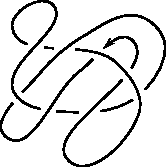
\includegraphics[width=1.5in]{8x_tref.pdf}
  \end{figure}
\end{frame}

\begin{frame}
  \frametitle{Natural questions about knot diagrams}
  \begin{block}{Question}
    What is the average minimal crossing \# of an 8-crossing diagram?\\
    \onslide<2>{\centering $0.52$}
  \end{block}
  \begin{figure}
    \centering
    \[
    \vcenter{\hbox{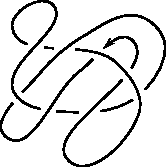
\includegraphics[width=1.5in]{8x_tref.pdf}}}
    \Rightarrow
    \vcenter{\hbox{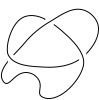
\includegraphics[width=1.5in]{8x_min_tref.pdf}}}
    \]
  \end{figure}
\end{frame}

\begin{frame}
  \frametitle{Natural questions about knot diagrams}
  \begin{definition}
    Define an operation on diagrams, \emph{untwisting}: Recursively RI
    untwist loops in a diagram until there are no more.
  \end{definition}

  \begin{figure}
    \centering
    \[
    \vcenter{\hbox{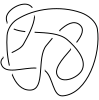
\includegraphics[width=1.5in]{8x_tref_loopy.pdf}}}
    \Rightarrow
    \vcenter{\hbox{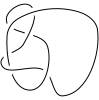
\includegraphics[width=1.5in]{8x_tref_deloopy.pdf}}}
    \]
  \end{figure}

\end{frame}

\begin{frame}
  \frametitle{Natural questions about knot diagrams}
  \begin{block}{Question}
    What is the average crossing \# of a untwisted 8-crossing diagram?\\
    \onslide<2>{\centering $2.20$}
  \end{block}
  \begin{figure}
    \centering
    \[
    \vcenter{\hbox{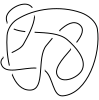
\includegraphics[width=1.5in]{8x_tref_loopy.pdf}}}
    \Rightarrow
    \vcenter{\hbox{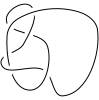
\includegraphics[width=1.5in]{8x_tref_deloopy.pdf}}}
    \]
  \end{figure}
\end{frame}

\begin{frame}
  \frametitle{Natural questions about knot diagrams}
  \begin{block}{Question}
    How many 8-crossing diagrams can be untwisted to the unknot?\\
    \onslide<2>{\centering $42.05\%$}
  \end{block}
  \begin{figure}
    \centering
    \includegraphics[width=1.5in]{tree_like_8x.pdf}
  \end{figure}
\end{frame}

\subsection{Background}

\begin{frame}
  \frametitle{Ansatz}
  \begin{figure}
    \centering
    \begin{tikzpicture}[->,,shorten >=1pt,semithick,align=center]
      % \tikzstyle{every node}=[align=center]
      \node[text width=1in] (plantri)
      {Polymers\\\includegraphics[width=.95in]{dna.jpg}};
      \node[text width=1in,right=.3in of plantri]  (expand)
      {Random curves\\\includegraphics[width=.95in]{space_polygon.jpg}};
      \node[text width=1in,right=.3in of expand] (isomch)
      {Knots\\\includegraphics[width=.95in]{knot_3d.jpg}};

      \path (plantri)    edge (expand)
      (expand)     edge (isomch);
    \end{tikzpicture}
  \end{figure}
\end{frame}

\begin{frame}
  \frametitle{Combinatorial approaches}
    \begin{figure}
    \centering
    \begin{tikzpicture}[->,,shorten >=1pt,semithick,align=center]
      % \tikzstyle{every node}=[align=center]
      \node[text width=1in] (plantri)
      {Polymers\\\includegraphics[width=.95in]{dna.jpg}};
      \node[text width=1in,right=.3in of plantri]  (expand)
      {Random curves\\\includegraphics[width=.95in]{space_polygon.jpg}};
      \node[text width=1in,right=.3in of expand] (isomch)
      {Knots\\\includegraphics[width=.95in]{knot_3d.jpg}};
      \node[text width=1in,below=.3in of isomch]  (combinatorics)
      {Random combinatorial\\
        \resizebox{.95in}{!}{
          \tikz[thick]{
            \foreach \x in {0,1,...,4} {
              % \draw[white,-,line width = 5] (\x*288-54:3) -- (\x*288+90:3);
              \draw[>=triangle 90 cap,white,<->,line width = 6,shorten >=3, shorten <=3] (\x*288-54:3) -- (\x*288+90:3);
              \draw[black,decoration={markings,mark=at position 0.25 with {\arrow{>}}},postaction={decorate}] (\x*288-54:3) -- (\x*288+90:3); }
            \foreach \x in {0,1,...,4} {
              \draw (\x*144-54:3)+(\x*144+99:1) node[auto,scale=0.7] {\x};}
            %\foreach \p/\x in {24/0,03/1,14/2,02/3,13/4} \node[scale=0.7] at (\x*144-90:1.5){$p_{\p}$};
            %\filldraw (306:3) circle (2pt);
            % \draw[step=0.5,gray,very thin] (-3,-3) grid (3,3);
            \pgfresetboundingbox \clip (-3,-2.75) rectangle (3,3);
          }
        }
      };

      \path (plantri)    edge (expand)
      (expand)     edge (isomch);
      \path (combinatorics) edge (isomch);
    \end{tikzpicture}
  \end{figure}
\end{frame}

\begin{frame}
  \frametitle{The Petaluma model}
  Satisfying theorems have been proven for the Petaluma model
  \begin{figure}
    \centering
    \resizebox{.8\columnwidth}{!}{\begin{tabular}{ccc}
\tikz[thick]{
\foreach \angle in {0, 72, ..., 288} \draw[decoration={markings,mark=at position 0.7 with {\arrow{>}}},postaction={decorate}] (0,0) .. controls +(\angle+36:4) and +(\angle:4) .. (0,0);
\filldraw (0,0)+(306:2.83) circle (2pt);
\foreach \angle/\num in {0/4, 72/3, 144/2, 216/1, 288/0} \draw (0,0)+(\angle-6:1) node[scale=1] {$\num$};
%\draw[step=0.5,gray,very thin] (-3,-3) grid (3,3);
\pgfresetboundingbox \clip (-3,-2.75) rectangle (3,3);} &
\tikz[thick]{
\draw[->,double,thick] (-0.5,-0.5) -- (0.5,-0.5);
%\draw[step=0.5,gray,very thin] (-0.5,-3) grid (0.5,3);
\pgfresetboundingbox \clip (-0.5,-2.75) rectangle (0.5,3);} &
\tikz[thick]{
\foreach \x in {0,1,...,4} {
%\draw[white,-,line width = 5] (\x*288-54:3) -- (\x*288+90:3);
\draw[>=triangle 90 cap,white,<->,line width = 6,shorten >=3, shorten <=3] (\x*288-54:3) -- (\x*288+90:3);
\draw[black,decoration={markings,mark=at position 0.25 with {\arrow{>}}},postaction={decorate}] (\x*288-54:3) -- node[fill=white,draw,circle,scale=0.6]{\x} (\x*288+90:3); }
\foreach \x in {0,1,...,4} {
\draw (\x*144-54:3)+(\x*144+99:1) node[auto,scale=0.7] {\x};}
\foreach \p/\x in {24/0,03/1,14/2,02/3,13/4} \node[scale=0.7] at (\x*144-90:1.5){$p_{\p}$};
\filldraw (306:3) circle (2pt);
%\draw[step=0.5,gray,very thin] (-3,-3) grid (3,3);
\pgfresetboundingbox \clip (-3,-2.75) rectangle (3,3);
} \\
Petal diagram & & Star diagram
\end{tabular}}

    (Diagram from Evan-Zohar, Hass, et al.)
    \label{fig:petaluma}
  \end{figure}
\end{frame}

\begin{frame}
  %\frametitle{The void}
  %There is no clear connection between the two models: E.g.\ how to
  %produce a star diagram from a random polygon?
  % \begin{figure}
  %   \centering
  %   \begin{tikzpicture}[->,,shorten >=1pt,semithick,align=center]
  %     % \tikzstyle{every node}=[align=center]
  %     \node[text width=1in,draw=black] (knots) {Knot types};
  %     \node[below=.5in of knots] (diagrams) {};
  %     \node[text width=1.2in,draw=black,left=.5in of diagrams] (curves) {Curve\\distributions};
  %     \node[text width=1.2in,draw=black,right=.5in of diagrams]  (combs)
  %     {Combinatorial distributions};

  %     \path (curves) edge (knots)
  %            (combs) edge (knots);
  %     \draw[-,decorate, decoration={zigzag}] (curves) -- (combs) node[midway,above]  {???};
  %     %\path (plantri)    edge (expand)
  %     %(expand)     edge (isomch);
  %   \end{tikzpicture}
  %   \caption{There is no convenient middle between the two methods}
  % \end{figure}
    \begin{figure}
    \centering
    \begin{tikzpicture}[->,,shorten
      >=1pt,semithick,align=center,minimum height=1.3in]
      % \tikzstyle{every node}=[align=center]
      \node[text width=1in] (plantri)
      {Polymers\\\includegraphics[width=.95in]{dna.jpg}};
      \node[text width=1in,right=.3in of plantri]  (expand)
      {Random curves\\\includegraphics[width=.95in]{space_polygon.jpg}};
      \node[text width=1in,right=.3in of expand] (isomch)
      {Knots\\\includegraphics[width=.95in]{knot_3d.jpg}};
      \node[fill=black,text=white,text width=1in,below=.3in of expand] (diagrams)
      {???};
      \node[text width=1in,below=.3in of isomch]  (combinatorics)
      {Random combinatorial\\
        \resizebox{.95in}{!}{
          \tikz[thick]{
            \foreach \x in {0,1,...,4} {
              % \draw[white,-,line width = 5] (\x*288-54:3) -- (\x*288+90:3);
              \draw[>=triangle 90 cap,white,<->,line width = 6,shorten >=3, shorten <=3] (\x*288-54:3) -- (\x*288+90:3);
              \draw[black,decoration={markings,mark=at position 0.25 with {\arrow{>}}},postaction={decorate}] (\x*288-54:3) -- (\x*288+90:3); }
            \foreach \x in {0,1,...,4} {
              \draw (\x*144-54:3)+(\x*144+99:1) node[auto,scale=0.7] {\x};}
            %\foreach \p/\x in {24/0,03/1,14/2,02/3,13/4} \node[scale=0.7] at (\x*144-90:1.5){$p_{\p}$};
            %\filldraw (306:3) circle (2pt);
            % \draw[step=0.5,gray,very thin] (-3,-3) grid (3,3);
            \pgfresetboundingbox \clip (-3,-2.75) rectangle (3,3);
          }
        }
      };

      \path (plantri)    edge (expand)
      (expand)     edge (isomch);
      \path (combinatorics) edge (isomch);
      \draw[<->] (expand) -- (diagrams);
      \draw[<->] (combinatorics) -- (diagrams);
    \end{tikzpicture}
  \end{figure}

\end{frame}

\begin{frame}
    \begin{figure}
      \vspace{-.05in}
    \centering
    \begin{tikzpicture}[->,,shorten
      >=1pt,semithick,align=center,minimum height=1.4in]
      % \tikzstyle{every node}=[align=center]
      \node[text width=1in] (plantri)
      {Polymers\\\includegraphics[width=.95in]{dna.jpg}};
      \node[text width=1in,right=.3in of plantri]  (expand)
      {Random curves\\\includegraphics[width=.95in]{space_polygon.jpg}};
      \node[text width=1in,right=.3in of expand] (isomch)
      {Knots\\\includegraphics[width=.95in]{knot_3d.jpg}};
      \node[text width=1in,below=.3in of expand] (diagrams)
      {Random diagrams\\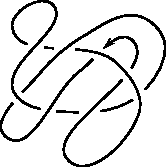
\includegraphics[width=.95in]{8x_tref.pdf}};
      \node[text width=1in,below=.3in of isomch]  (combinatorics)
      {Random combinatorial\\
        \resizebox{.95in}{!}{
          \tikz[thick]{
            \foreach \x in {0,1,...,4} {
              % \draw[white,-,line width = 5] (\x*288-54:3) -- (\x*288+90:3);
              \draw[>=triangle 90 cap,white,<->,line width = 6,shorten >=3, shorten <=3] (\x*288-54:3) -- (\x*288+90:3);
              \draw[black,decoration={markings,mark=at position 0.25 with {\arrow{>}}},postaction={decorate}] (\x*288-54:3) -- (\x*288+90:3); }
            \foreach \x in {0,1,...,4} {
              \draw (\x*144-54:3)+(\x*144+99:1) node[auto,scale=0.7] {\x};}
            %\foreach \p/\x in {24/0,03/1,14/2,02/3,13/4} \node[scale=0.7] at (\x*144-90:1.5){$p_{\p}$};
            %\filldraw (306:3) circle (2pt);
            % \draw[step=0.5,gray,very thin] (-3,-3) grid (3,3);
            \pgfresetboundingbox \clip (-3,-2.75) rectangle (3,3);
          }
        }
      };

      \path (plantri)    edge (expand)
      (expand)     edge (isomch);
      \path (combinatorics) edge (isomch);
      \draw[<->] (expand) -- (diagrams);
      \draw[<->] (combinatorics) -- (diagrams);
      \path (diagrams) edge (isomch);
    \end{tikzpicture}
  \end{figure}

  %\frametitle{The random diagram model}
  % Every space curve can
  % project to a diagram, \emph{and} diagrams are combinatorial objects.
  % \begin{figure}
  %   \centering
  %   \begin{tikzpicture}[->,,shorten >=1pt,semithick,align=center]
  %     % \tikzstyle{every node}=[align=center]
  %     \node[text width=1in,draw=black] (knots) {Knot types};
  %     \node[below=.5in of knots] (diagrams) {};
  %     \node[text width=1.2in,draw=black,left=.5in of diagrams] (curves) {Curve\\distributions};
  %     \node[text width=1.2in,draw=black,right=.5in of diagrams]
  %     (combs)
  %     {Combinatorial distributions};
  %     \node[text width=1.4in, draw=black,below=.3in of diagrams]
  %     (dias) {Random\\diagram model};

  %     \path (curves) edge (knots)
  %            (combs) edge (knots)
  %            (dias) edge (knots);

  %     \draw[<->,thick,beamerviolet] (dias.west) -- (curves);
  %     \draw[<->,thick,beamerviolet] (dias.east) -- (combs);
  %     %\path (plantri)    edge (expand)
  %     %(expand)     edge (isomch);
  %   \end{tikzpicture}
  %   \caption{We're trying to fill the void with the random diagram model}
  % \end{figure}
\end{frame}

\subsection{Tabulation}

\begin{frame}
  \frametitle{Random diagrams}
  \begin{definition}
    In the \emph{random diagram model} of random knotting, a
    $n$-crossing diagram is drawn uniformly from the finite set of
    $n$-crossing knot diagrams.
  \end{definition}
  \begin{figure}
    \centering
    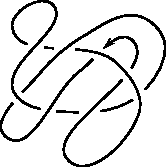
\includegraphics[width=1.2in]{8x_tref.pdf}\qquad
    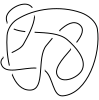
\includegraphics[width=1.2in]{8x_tref_loopy.pdf}\qquad
    \includegraphics[width=1.2in]{tree_like_8x.pdf}
  \end{figure}
\end{frame}

\begin{frame}
  \frametitle{Random diagrams}
  \begin{definition}
    A \emph{knot diagram} is a equivalence class of generic immersions of the oriented $S^1$ into
    the sphere $S^2$ together with over-under strand information at each
    double point up to diffeomorphism of $S^2$.
  \end{definition}
  \begin{figure}
    \centering
    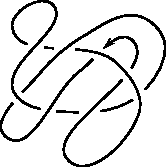
\includegraphics[width=1.2in]{8x_tref.pdf}\qquad
    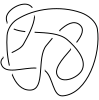
\includegraphics[width=1.2in]{8x_tref_loopy.pdf}\qquad
    \includegraphics[width=1.2in]{tree_like_8x.pdf}
  \end{figure}
\end{frame}

\begin{frame}
  \frametitle{How to enumerate knot diagrams}
  \begin{definition}
    A \emph{knot shadow} is a generic equivalence class of immersions of the unoriented $S^1$
    into the sphere $S^2$ up to diffeomorphism of $S^2$.
  \end{definition}
  \begin{enumerate}
  \item Enumerate shadows
  \item Assign crossing and orientation information and identify
    equivalent diagrams
  \end{enumerate}
\end{frame}

\begin{frame}
  \frametitle{Tabulating knot shadows}
  \begin{proposition}
    Knot shadows $\leftrightarrow$ 1-component 4-valent embedded
    planar multigraphs up to embedded isomorphism
  \end{proposition}
  \begin{enumerate}
  \item<2-> Add loops and edges to planar simple graphs
  \item<3-> Generate multiquadrangulations by connect sum, take
    dual graphs
  \end{enumerate}
  \vspace{-.3in}
  \begin{center}
    \begin{tabular}{ccccc}
      \onslide<2->{$\vcenter{\hbox{\includegraphics[width=.8in]{pre_shadow_graph.pdf}}}$}
      & \onslide<2->{$\Rightarrow$}
      & $\vcenter{\hbox{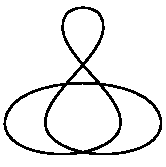
\includegraphics[width=.8in]{result_shadow.pdf}}}$
      & \onslide<3->{$\Leftarrow$}
      & \onslide<3->{$\vcenter{\hbox{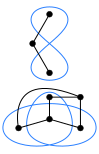
\includegraphics[width=.8in]{pre_shadow_quads.pdf}}}$}
    \end{tabular}
  \end{center}
  \onslide<4->{Actually generate all \textbf{link shadows}, then
    restrict to knot shadows}
\end{frame}

% \begin{frame}
%   \frametitle{From shadows to diagrams}
%   Expansion of $n$-crossing shadows to diagrams procedure:
%   \begin{enumerate}
%   \item Orient each component. (2 choices)
%   \item Assign over-under information to each
%     vertex. ($2^n$ choices)
%   \item Group diagrams by isomorphism.
%   \end{enumerate}
% \end{frame}


\begin{frame}
  \frametitle{Assign crossings, orientation, identify}
  \begin{enumerate}
  \item Orient each component. (2 choices)
  \item Assign over-under information to each
    vertex. ($2^n$ choices)
  \end{enumerate}
  \begin{table}
    \centering
    \begin{tabular}{r|ccc}
      \rowcolor{gray!50}
      n  & \# knot shadows & $2^{n+1}$ (\# shadows) & \# knot diagrams
      \\
      3  & 6               & 96               & 36                   \\
      4  & 19              & 608              & 276                  \\
      5  & 76              & 4,864            & 2,936                \\
      6  & 376             & 48,128           & 35,872               \\
      7  & 2,194           & 561,664          & 484,088              \\
      8  & 14,614          & 7,482,368        & 6,967,942            \\
      9  & 106,421         & 108,975,104      & 105,555,336          \\
    \end{tabular}
    \label{tab:counts}
  \end{table}
\end{frame}

\begin{frame}
  \frametitle{Verifying against existing shadow counts}
  \begin{columns}
    \begin{column}[T]{.6\columnwidth}
      \centering
      \includegraphics[width=\columnwidth]{arnold_table.png}\\
      {\small V.I. Arnol'd. \textit{Topological Invariants of Plane Curves}}
      \hfill\\\hfill\\
      \includegraphics[width=\columnwidth]{oeis_shadows.png}\\
      {\small OEIS A008989}
    \end{column}
    \begin{column}[T]{.4\columnwidth}
          %\begin{table}
            \centering
            \begin{tabular}{r|c}
              \rowcolor{gray!50}
              n & \# knot shadows \\
              \rowcolor{yellow!40}
              0 & 1 \\
              \rowcolor{yellow!40}
              1 & 1 \\
              \rowcolor{yellow!40}
              2 & 2 \\
              \rowcolor{yellow!40}
              3 & 6 \\
              \rowcolor{yellow!40}
              4 & 19\\
              \rowcolor{yellow!40}
              5 & 76 \\
              \rowcolor{yellow!40}
              6 & 376 \\
              \rowcolor{yellow!40}
              7 & 2194 \\
              8 & 14614 \\
              9 & 106421 \\
            \end{tabular}
            \label{tab:counts}
          %\end{table}
        \end{column}
  \end{columns}
  We have not found any existing counts of \emph{diagrams}.
\end{frame}

% \begin{frame}
%   \frametitle{How many link shadows?}
%   \begin{block}{}
%     Counts of link shadows with $n$ crossings match K\'apolnai,
%     Domokos, and Szab\'o's counts of spherical multiquadrangulations
%     with $n+2$ crossings (hence $n$ faces).
%   \end{block}

%     \textit{Caveat:} They use \texttt{plantri} in their
%       computations too, although it is not clear how.

% \end{frame}

% \begin{frame}
%   \frametitle{How many knot shadows?}
%   \begin{block}{}
%     Counts of knot shadows with $n$ crossings match Arnol'd's counts of
%     immersions of the unoriented circle into the unoriented sphere
%     with $n$ double points (OEIS A008989).
%   \end{block}

%     \textit{Caveat:} Arnol'd's list is for $n=0$ to $n=5$; the
%       terms for $n=6$ and $n=7$ are attributed to Guy H.\ Valette with
%       no clear source.
% \end{frame}

% \begin{frame}
%   \frametitle{How many shadows?}
%     \begin{table}
%     \centering
%     \begin{tabular}{r|c}
%       n & \# knot shadows \\
%       \hline
%       0 & 1 \\
%       1 & 1 \\
%       2 & 2 \\
%       3 & 6 \\
%       4 & 19\\
%       5 & 76 \\
%       6 & 376$^{*}$ \\
%       7 & 2194$^{*}$ \\
%       8 & 14614$^{**}$ \\
%       9 & 106421$^{**}$ \\
%     \end{tabular}
%     \caption{$*$: Attributed to Guy H.\
%       Valette. $**$: New; values not in OEIS.}
%     \label{tab:counts}
%   \end{table}
% \end{frame}

% \begin{frame}
%   \frametitle{Duals to quadrangulations}
%   \begin{figure}
%     \hphantom{.}
%     \hfill
%     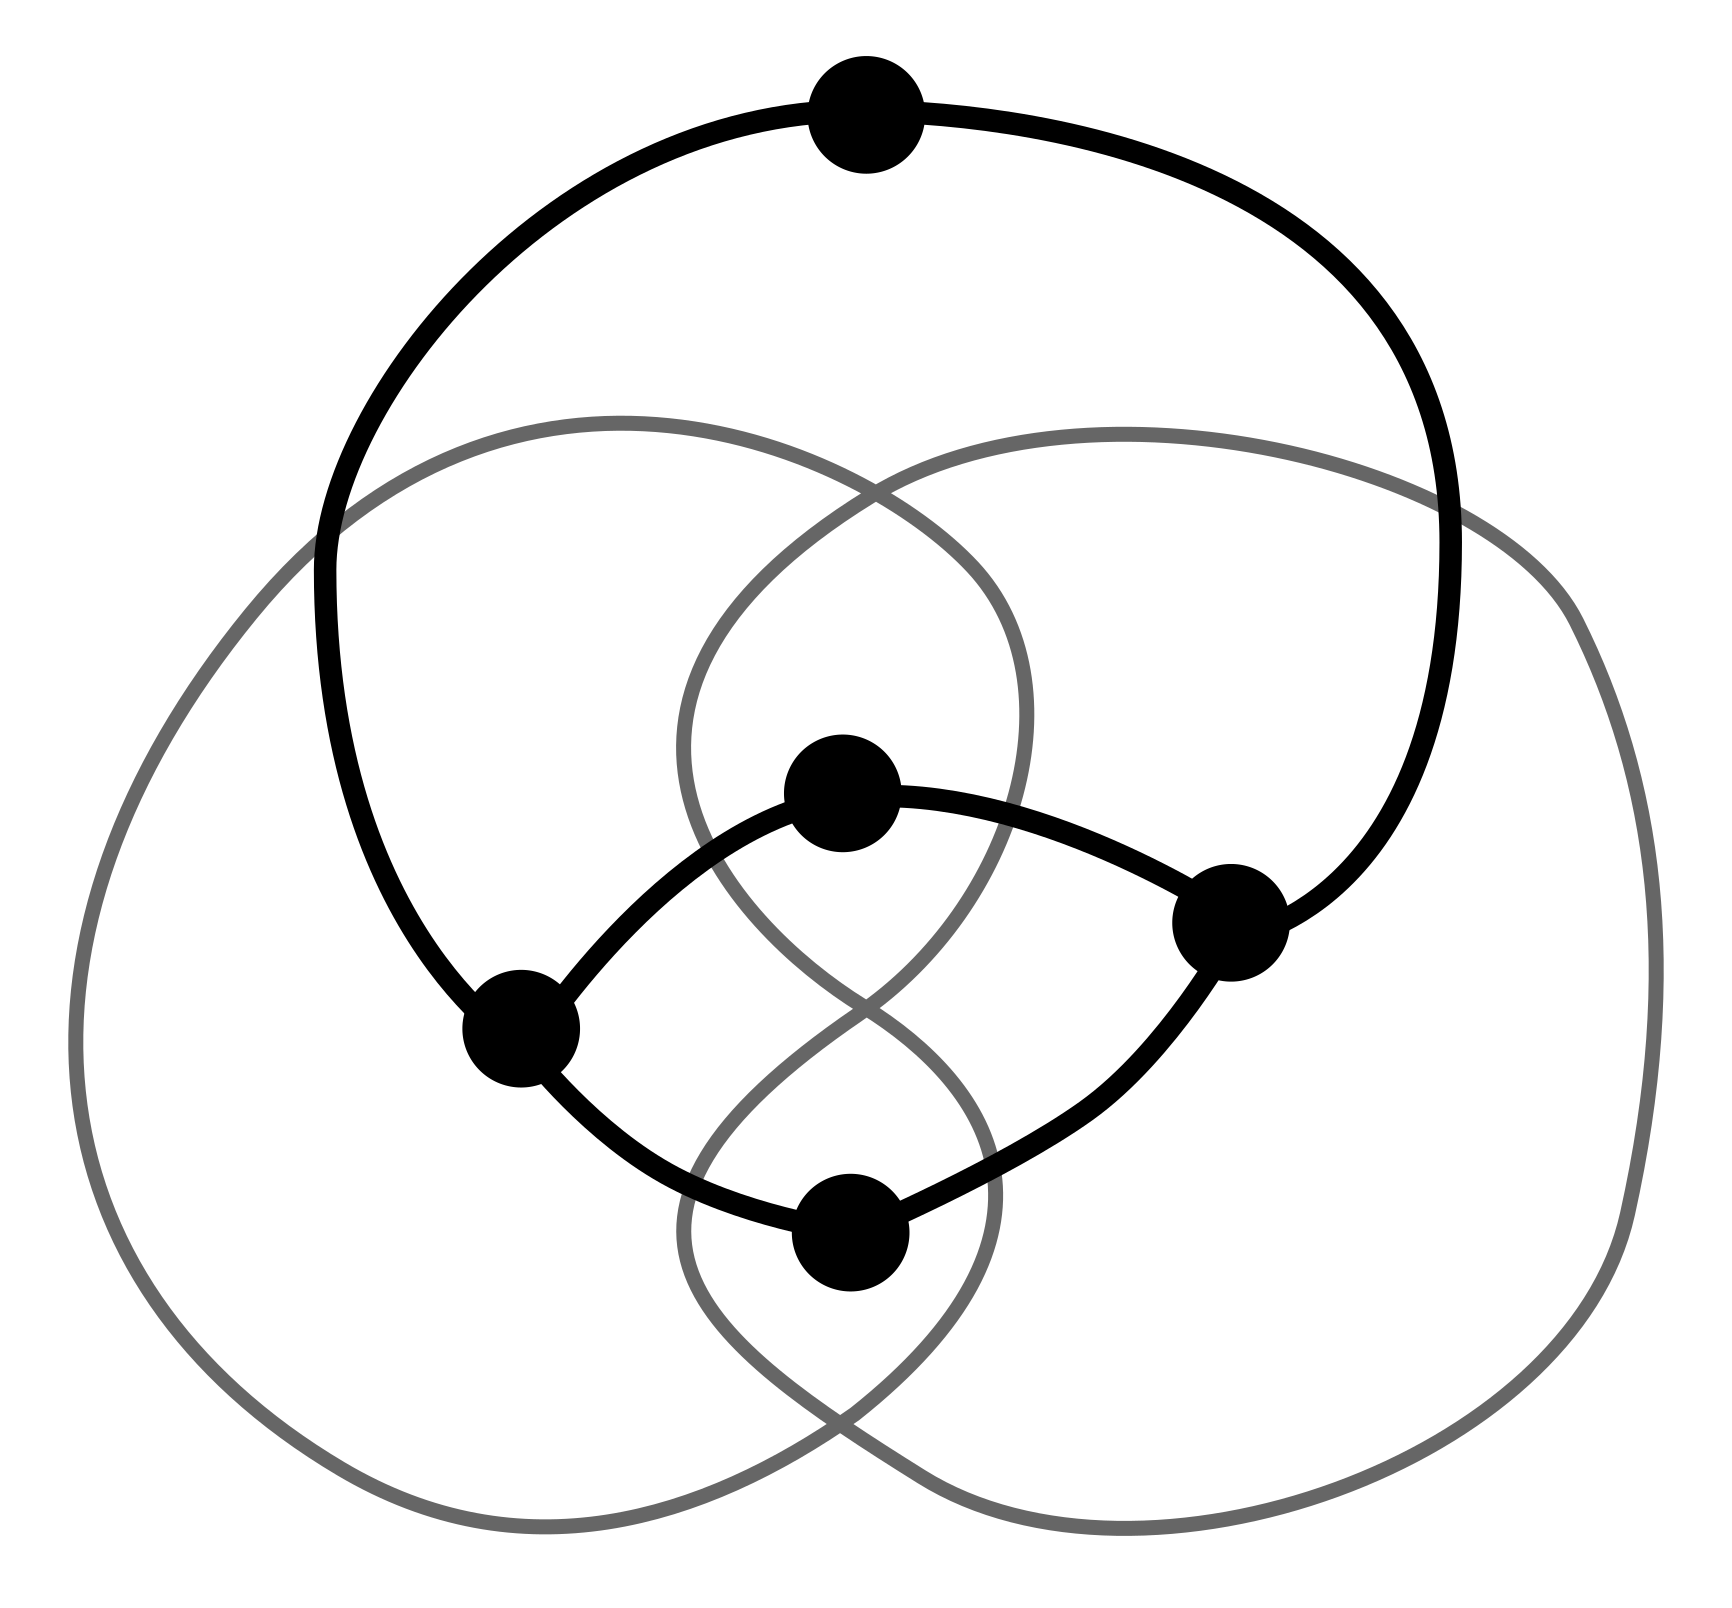
\includegraphics[height=1.25in]{quadrangulation} \hfill
%     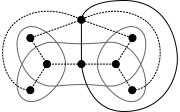
\includegraphics[height=1.25in]{non-simple-quadrangulation}
%     \hfill
%     \hphantom{.}
%     \caption{\label{fig:NonSimpleQuad} Find all quadrangulations of
%     the sphere in $n$ faces. Shadows are dual to quadrangulations.}
%   \end{figure}
% \end{frame}

% \begin{frame}
%   \frametitle{Planar graph expansions}
%   \begin{figure}
%     \centering
%       \includegraphics[width=4in]{expansion-from-simple-graph.pdf}
%     \caption{Reduction to a planar graph of degree $\le 4$ and
%       connectivity $\ge 1$. Expansion is the inverse.}
%     \label{fig:graphexpand}
%   \end{figure}
% \end{frame}

\begin{frame}[label=knotspace1]
  \frametitle{The space of shadows}
  \begin{figure}
    \centering
    \includegraphics[width=\textwidth,height=\textheight,keepaspectratio]{epsgroup_0_collage.eps}
    \\ Link shadows. Pictures generated by Eric Lybrand (UGA
      undergrad).
    \label{fig:planarcollage0}
  \end{figure}
\end{frame}

\begin{frame}[label=knotspace2]
  \frametitle{The space of shadows}
  \begin{figure}
    \centering
    \includegraphics[width=\textwidth,height=\textheight,keepaspectratio]{epsgroup_1_collage.eps}
     \\ Link shadows. Pictures generated by Eric Lybrand (UGA
      undergrad).
    \label{fig:planarcollage1}
  \end{figure}
\end{frame}

\begin{frame}
  \frametitle{The space of shadows}
  \begin{figure}
    \centering
    \includegraphics[width=\textwidth,height=\textheight,keepaspectratio]{epsgroup_10_collage.eps}
 \\ Link shadows. Pictures generated by Eric Lybrand (UGA
      undergrad).
    \label{fig:planarcollage10}
  \end{figure}
\end{frame}

\begin{frame}
  \frametitle{The space of shadows}
  \begin{figure}
    \centering
    \includegraphics[width=\textwidth,height=\textheight,keepaspectratio]{epsgroup_16_collage.eps}
  \\ Link shadows. Pictures generated by Eric Lybrand (UGA
      undergrad).
    \label{fig:planarcollage16}
  \end{figure}
\end{frame}

\begin{frame}
  \frametitle{Tabulation is difficult!}
  Accounting for symmetry is complicated.

  \begin{figure}
    \centering
    \begin{tabular}{ccc}
      \begin{overpic}[width=1.2in]{shadow_skinny.pdf}
        \put(77,45){1}
        \put(17,45){2}
        \put(47,10){3}
      \end{overpic}
      & \hspace{.5in} & 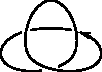
\includegraphics[width=1.2in]{tref_isom_1.pdf}
      \\ \rowcolor{white}&& \\
      \begin{overpic}[width=1.2in]{shadow_skinny.pdf}
        \put(77,45){2}
        \put(17,45){1}
        \put(47,10){3}
      \end{overpic}
      & \hspace{.5in} & \includegraphics[width=1.2in]{tref_isom_2.pdf} \\

    \end{tabular}
    \label{fig:trefsym}
  \end{figure}
\end{frame}

\begin{frame}
  \frametitle{Breaking symmetries could make counting easier}
  \begin{figure}
    \centering
    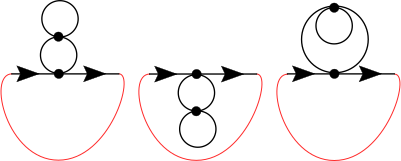
\includegraphics[width=.8\columnwidth]{legdias.pdf}
    \label{fig:legdia}
  \end{figure}

  Two-leg diagrams counted by generating function (Bouttier,
  et al.\ 2003):
  \[ G_0 = \frac{24g - 1 + \sqrt{1-12g}}{9g(1+\sqrt{1-12g})} = 1 + 2g
  + 9g^2 + 54g^3 + 378g^4 +  \cdots \]
\end{frame}

\section{Data and Analysis}

\subsection{Data}

% \begin{frame}
%   \frametitle{Knotting probabilities}
%   \begin{itemize}
%   \item Able to run searches across entire space computationally.
%   \item Can check knot type of each diagram (HOMFLY is typically
%     enough for our low crossing number)
%   \item Possible to run many different types of searches
%   \end{itemize}

% \end{frame}

\begin{frame}
  \frametitle{Knotting in diagrams}
  \begin{figure}
    \centering
    \begin{tikzpicture}[scale=1]
      \begin{axis}[
        %ymode=log,
        %log ticks with fixed point,
        title={Ratios of knots in $n$-crossing diagrams},
        xlabel={\# crossings in diagram},
        ylabel={Ratios of knots},
        cycle list name=Mark-Set1-9,
        legend pos=outer north east,
        legend entries={$3_1$, $4_1$, $5_1$, $5_2$, $0_1$},
        ymin=0, ymax=1,
        ]
        \addplot table[x=n,y=3.1] {knot_freq.tsv};
        \addplot table[x=n,y=4.1] {knot_freq.tsv};
        \addplot table[x=n,y=5.1] {knot_freq.tsv};
        \addplot table[x=n,y=5.2] {knot_freq.tsv};
        \addplot table[x=n,y=0.1] {knot_freq.tsv};
      \end{axis}
    \end{tikzpicture}
    \label{fig:kgrow1}
  \end{figure}
\end{frame}


\begin{frame}
  \begin{figure}
    \centering
    \begin{tikzpicture}[scale=1]
      \begin{axis}[
        ymode=log,
        log ticks with fixed point,
        title={Ratios of knots in $n$-crossing diagrams (log scale)},
        xlabel={\# crossings in diagram},
        ylabel={Ratios of knots},
        cycle list name=Mark-Set1-9,
        legend pos=south west,
        legend entries={$3_1$, $4_1$, $5_1$, $5_2$},
        ]
        \addplot table[x=n,y=3.1] {knot_freq.tsv};
        \addplot table[x=n,y=4.1] {knot_freq.tsv};
        \addplot table[x=n,y=5.1] {knot_freq.tsv};
        \addplot table[x=n,y=5.2] {knot_freq.tsv};
      \end{axis}
    \end{tikzpicture}
    \label{fig:kgrow1}
  \end{figure}
\end{frame}


\begin{frame}
  \begin{figure}
    \centering
      \tikzset{mark=*}
    \begin{tikzpicture}[scale=1]
      \begin{axis}[
        ymode=log,
        log ticks with fixed point,
        title={Ratios of knots in $n$-crossing diagrams (log scale)},
        xlabel={\# crossings in diagram},
        ylabel={Ratios of knots},
        cycle list name=Mark-Set1-9,
        legend style={font=\tiny},
        legend pos=outer north east,
        legend entries={$3_1$, $4_1$, $5_1$, $5_2$, $6_1$, $6_2$, $3_1
          \# 3_1$, $3_1 \# 3_1^*$, $7_1$, $7_2$, $7_3$, $7_4$, $7_5$,
          $7_6$, $7_7$},
        ]
        \addplot table[x=n,y=3.1] {knot_freq.tsv};
        \addplot table[x=n,y=4.1] {knot_freq.tsv};
        \addplot table[x=n,y=5.1] {knot_freq.tsv};
        \addplot table[x=n,y=5.2] {knot_freq.tsv};
        \addplot table[x=n,y=6.1] {knot_freq.tsv};
        \addplot table[x=n,y=6.2] {knot_freq.tsv};
        \addplot table[x=n,y=3.1c3.1] {knot_freq.tsv};
        \addplot table[x=n,y=3.1c3.1m] {knot_freq.tsv};
        \addplot table[x=n,y=7.1] {knot_freq.tsv};
        \addplot table[x=n,y=7.2] {knot_freq.tsv};
        \addplot table[x=n,y=7.3] {knot_freq.tsv};
        \addplot table[x=n,y=7.4] {knot_freq.tsv};
        \addplot table[x=n,y=7.5] {knot_freq.tsv};
        \addplot table[x=n,y=7.6] {knot_freq.tsv};
        \addplot table[x=n,y=7.7] {knot_freq.tsv};
      \end{axis}
    \end{tikzpicture}

    \label{fig:kgrow2}
  \end{figure}
\end{frame}

\begin{frame}
  \frametitle{A question on unknotting}
  \begin{theorem}[(Frisch-Wassermann-Delbr\"uck Conjecture) Sumners-Whittington 1988]
    The ratio of unknots in random $n$-edge self-avoiding lattice
    polygons tends to zero exponentially with $n$.
  \end{theorem}
  \begin{block}{Conjecture}
    The ratio of unknots in diagrams tends to zero as $n$
    increases. (Exponentially?)
  \end{block}
  Exist theorems on planar (simple) graphs (Dowden 2008) similar to
  the Kesten pattern theorem (Kesten 1963) for lattice walks
\end{frame}

\begin{frame}
  \begin{figure}
    \centering
    \begin{tikzpicture}[scale=1]
      \begin{axis}[
        %ymode=log,
        %log ticks with fixed point,
        title={Ratio of unknots in $n$-crossing diagrams},
        xlabel={\# crossings in diagram},
        ylabel={Ratio of unknots},
        cycle list name=Mark-Set1-9,
        legend pos=south west,
        legend entries={Unknots},
        ymax=1, ymin=0,
        ]
        \addplot table[x=n,y=0.1] {knot_freq.tsv};
      \end{axis}
    \end{tikzpicture}
    \label{fig:unkdecay}
  \end{figure}
\end{frame}


\begin{frame}
  \begin{figure}
    \centering
    \begin{tikzpicture}[scale=1]
      \begin{axis}[
        ymode=log,
        log ticks with fixed point,
        title={Ratio of unknots in $n$-crossing diagrams (log scale)},
        xlabel={\# crossings in diagram},
        ylabel={Ratio of unknots},
        cycle list name=Mark-Set1-9,
        legend pos=south west,
        legend entries={Unknots},
        ymax=1,
        ]
        \addplot table[x=n,y=0.1] {knot_freq.tsv};
      \end{axis}
    \end{tikzpicture}
    \label{fig:unkdecay}
  \end{figure}
\end{frame}


% \begin{frame}
%   \frametitle{Counting monogons and bigons in knot shadows}
%     \begin{table}
%     \centering
%     \resizebox{\columnwidth}{!}{\begin{tabular}{r|ccccc}
%                                   \rowcolor{gray!50}
%       $n$ & shadows & 1-gon & 2-gon & neither \\
%       3 & 6 & 5 (83.33\%) & 3 (50\%) & 0 \\
%       4 & 19 & 18 (94.74\%) & 11 (57.89\%) & 0 \\
%       5 & 76 & 74 (97.37\%) & 52 (68.42\%) & 0 \\
%       6 & 376 & 371 (98.67\%) & 275 (73.14\%) & 0 \\
%       7 & 2,194 & 2,178 (99.27\%) & 1,714 (78.12\%) & 0 \\
%       8 & 14,614 & 14,562 (99.64\%) & 11,892 (81.37\%) & 1 \\
%       9 & 106,421 & 106,216 (99.81\%) & 89,627 (84.22\%) & 1 \\
%     \end{tabular}}
%     \label{tab:counts}
%   \end{table}
% \end{frame}

\begin{frame}[label=knotspace1]
  \frametitle{Why so many unknots?}
  \begin{figure}
    \centering
    \includegraphics[width=\textwidth,height=\textheight,keepaspectratio]{epsgroup_0_collage.eps}
    \\ Link shadows. Pictures generated by Eric Lybrand (UGA
      undergrad).
    \label{fig:planarcollage0}
  \end{figure}
\end{frame}

\begin{frame}[label=knotspace2]
  \frametitle{Why so many unknots?}
  \begin{figure}
    \centering
    \includegraphics[width=\textwidth,height=\textheight,keepaspectratio]{epsgroup_1_collage.eps}
     \\ Link shadows. Pictures generated by Eric Lybrand (UGA
      undergrad).
    \label{fig:planarcollage1}
  \end{figure}
\end{frame}


\begin{frame}
    \begin{figure}
    \centering
    \begin{tikzpicture}[scale=1]
      \begin{axis}[
        ybar stacked,
        %stack plots=y,
        bar width=.5,
        area style,
        cycle multi list={OrRd-9},
        title={Reidemeister-I loops (monogons) in diagrams},
        xlabel={\# crossings in diagram},
        legend style={font=\tiny},
        legend pos=outer north east,
        legend entries={0,1,2,3,4,5,6,7,8,9},
        ylabel={Ratio},
        ymin=0, ymax=1,
        ]
        \addplot table[x=n,y=0] {mono_counts.tsv};% \closedcycle;
        \addplot table[x=n,y=1] {mono_counts.tsv};% \closedcycle;
        \addplot table[x=n,y=2] {mono_counts.tsv};% \closedcycle;
        \addplot table[x=n,y=3] {mono_counts.tsv};% \closedcycle;
        \addplot table[x=n,y=4] {mono_counts.tsv};% \closedcycle;
        \addplot table[x=n,y=5] {mono_counts.tsv};% \closedcycle;
        \addplot table[x=n,y=6] {mono_counts.tsv};% \closedcycle;
        \addplot table[x=n,y=7] {mono_counts.tsv};% \closedcycle;
        \addplot table[x=n,y=8] {mono_counts.tsv};% \closedcycle;
        \addplot table[x=n,y=9] {mono_counts.tsv};% \closedcycle;
        %\addplot table[x=n,y=10] {mono_bi_counts.tsv};% \closedcycle;
      \end{axis}
    \end{tikzpicture}
    \label{fig:monogons}
  \end{figure}
\end{frame}

\begin{frame}
    \begin{figure}
    \centering
    \begin{tikzpicture}[scale=1]
      \begin{axis}[
        ybar stacked,
        %stack plots=y,
        bar width=.5,
        area style,
        cycle multi list={OrRd-9},
        title={Bigons in diagrams},
        xlabel={\# crossings in diagram},
        legend style={font=\tiny},
        legend pos=outer north east,
        legend entries={0,1,2,3,4,5,6,7,8,9},
        ylabel={Ratio},
        ymin=0, ymax=1,
        ]
        \addplot table[x=n,y=0] {bi_counts.tsv};% \closedcycle;
        \addplot table[x=n,y=1] {bi_counts.tsv};% \closedcycle;
        \addplot table[x=n,y=2] {bi_counts.tsv};% \closedcycle;
        \addplot table[x=n,y=3] {bi_counts.tsv};% \closedcycle;
        \addplot table[x=n,y=4] {bi_counts.tsv};% \closedcycle;
        \addplot table[x=n,y=5] {bi_counts.tsv};% \closedcycle;
        \addplot table[x=n,y=6] {bi_counts.tsv};% \closedcycle;
        \addplot table[x=n,y=7] {bi_counts.tsv};% \closedcycle;
        \addplot table[x=n,y=8] {bi_counts.tsv};% \closedcycle;
        \addplot table[x=n,y=9] {bi_counts.tsv};% \closedcycle;
        %\addplot table[x=n,y=10] {bi_bi_counts.tsv};% \closedcycle;
      \end{axis}
    \end{tikzpicture}
    \label{fig:bigons}
  \end{figure}
\end{frame}


\begin{frame}
  \frametitle{Basic polyhedra $8^*$ and $9^*$}
  \begin{proposition}
    Conway's basic polyhedra $8^*$ and $9^*$ are the only diagrams in
    $\le 9$ crossings with no monogons or bigons.
  \end{proposition}
  \begin{figure}
    \centering
    \includegraphics[width=.3\columnwidth]{8_18_celtic.png}\hspace{.1\columnwidth}
    \includegraphics[width=.3\columnwidth]{9_40_symmetric.png}
    \\{\centering $8_{18}$ (left), $9_{40}$ (right).}
    \label{fig:basicpoly}
  \end{figure}
\end{frame}

\begin{frame}
  \frametitle{Some shadows are always unknots}
  A \emph{tree-like curve} (Aicardi 1994) is a knot shadow which can be untwisted to
  the trivial shadow.
  \begin{figure}
    \centering
    \includegraphics[width=1.5in]{tree_like_8x.pdf}
    \label{fig:treelike}
  \end{figure}
  Tree-like curves $\Rightarrow$ lower bound on unknottedness.
\end{frame}

% \begin{frame}
%   \frametitle{Tree-like curves}
%     \begin{table}
%     \centering
%     \begin{tabular}{r|ccc}
%       \rowcolor{gray!50}
%       n & \# knot shadows & \# tree-like & \% tree-like \\
%       1 & 1               & 1            & 100.00\%     \\
%       2 & 2               & 2            & 100.00\%     \\
%       3 & 6               & 5            & 88.88\%      \\
%       4 & 19              & 16           & 86.23\%      \\
%       5 & 76              & 55           & 74.39\%      \\
%       6 & 376             & 240          & 63.12\%      \\
%       7 & 2,194           & 1149         & 51.92\%      \\
%       8 & 14,614          & 6,229        & 42.05\%      \\
%       9 & 106,421         & 35,995       & 33.54\%      \\
%     \end{tabular}
%     \label{tab:counts}
%   \end{table}
% \end{frame}

\begin{frame}
  \begin{figure}
    \centering
    \begin{tikzpicture}[scale=1]
      \begin{axis}[
        %ymode=log,
        %log ticks with fixed point,
        title={Ratio of unknots, tree-like curves in $n$-crossing diagrams},
        xlabel={\# crossings in diagram},
        ylabel={Percent},
        legend style={font=\tiny},
        legend pos=south west,
        cycle list name=Mark-Set1-9,
        legend entries={Unknots, Tree-like},
        ymin=0, ymax=1
        ]
        \addplot table[x=n,y=0.1] {knot_freq.tsv};
        \addplot table[x=n,y=diarat] {treelike.tsv};
      \end{axis}
    \end{tikzpicture}
    \label{fig:unkdecay}
  \end{figure}
\end{frame}

\begin{frame}
  \begin{figure}
    \vspace{-.2in}
    \centering
    \begin{tikzpicture}[scale=1]
      \begin{axis}[
        ymode=log,
        log ticks with fixed point,
        title={Ratio of unknots, tree-like curves in $n$-crossing diagrams (log scale)},
        xlabel={\# crossings in diagram},
        ylabel={Percent},
        legend style={font=\tiny},
        legend pos=south west,
        cycle list name=Mark-Set1-9,
        legend entries={Unknots, Tree-like}
        ]
        \addplot table[x=n,y=0.1] {knot_freq.tsv};
        \addplot table[x=n,y=diarat] {treelike.tsv};
      \end{axis}
    \end{tikzpicture}
    Tree-like curves alone explain only some of the unknot fraction
    \label{fig:unkdecay}
  \end{figure}
\end{frame}

\begin{frame}
  \begin{figure}
    \centering
    \begin{tikzpicture}[scale=1]
      \begin{axis}[
        title={Crossing \# vs. Average untwisted crossing \#},
        xlabel={\# crossings in diagram},
        ylabel={Average \# crossings in untwisted diagram},
        cycle list name=Mark-Set1-9,
        ymin=0, ymax=9,
        ]
        \addplot table[x=n,y=avg] {avgcn_counts.tsv};
      \end{axis}
    \end{tikzpicture}
    \label{fig:unkdecay}
  \end{figure}
\end{frame}

\begin{frame}
    \begin{figure}
    \centering
    \begin{tikzpicture}[scale=1]
      \begin{axis}[
        ybar stacked,
        %stack plots=y,
        bar width=.5,
        area style,
        cycle multi list={OrRd-9},
        title={Untwisted crossing \#},
        xlabel={\# crossings in diagram},
        legend style={font=\tiny},
        legend pos=outer north east,
        legend entries={0,1,2,3,4,5,6,7,8,9},
        ylabel={Ratio},
        ymin=0, ymax=1,
        ]
        \addplot table[x=n,y=0] {avgcn_counts.tsv};% \closedcycle;
        \addplot table[x=n,y=1] {avgcn_counts.tsv};% \closedcycle;
        \addplot table[x=n,y=2] {avgcn_counts.tsv};% \closedcycle;
        \addplot table[x=n,y=3] {avgcn_counts.tsv};% \closedcycle;
        \addplot table[x=n,y=4] {avgcn_counts.tsv};% \closedcycle;
        \addplot table[x=n,y=5] {avgcn_counts.tsv};% \closedcycle;
        \addplot table[x=n,y=6] {avgcn_counts.tsv};% \closedcycle;
        \addplot table[x=n,y=7] {avgcn_counts.tsv};% \closedcycle;
        \addplot table[x=n,y=8] {avgcn_counts.tsv};% \closedcycle;
        \addplot table[x=n,y=9] {avgcn_counts.tsv};% \closedcycle;
        %\addplot table[x=n,y=10] {mono_bi_counts.tsv};% \closedcycle;
      \end{axis}
    \end{tikzpicture}
    \label{fig:monogons}
  \end{figure}
\end{frame}

% \begin{frame}
%   \frametitle{Untwisted crossing number}
%   \begin{table}
%     \centering
%     \begin{tabular}{r|c}
%       \rowcolor{gray!50}
%       $n$ & Average untwisted crossing \# \\
%       3   & 0.50                         \\
%       4   & 0.53                         \\
%       5   & 0.92                         \\
%       6   & 1.25                         \\
%       7   & 1.72                         \\
%       8   & 2.19                         \\
%       9   & 2.70                         \\
%     \end{tabular}
%     \label{tab:untwist}
%   \end{table}
% \end{frame}


% \begin{frame}
%   \frametitle{Prime knot shadows}
%   How many diagrams are connect sums? Prime?  [Figure]
% \end{frame}

\subsection{Further questions}

\begin{frame}
  \frametitle{Questions to answer}
  Random curves project to diagrams.
  \begin{block}{Question}
    How does the pushforward measure differ from uniform diagram
    sampling? (c.f.\ Hua, Nguyen, Raghavan, Arsuaga, Vasquez 2005)
  \end{block}
  \begin{figure}
    \centering
    \begin{tabular}{ccc}
      $\vcenter{\hbox{\includegraphics[width=1.5in]{shonk_spacepoly.png}}}$
      & $\stackrel{\pi}{\rightarrow}$
      & $\vcenter{\hbox{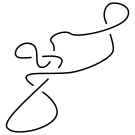
\includegraphics[width=1.5in]{shonk_as_diagram.pdf}}}$
    \end{tabular}
\end{figure}
(from Shonkwiler)

\end{frame}

\begin{frame}
  \frametitle{Questions to answer}
  \begin{block}{Question}
    Let $PD(n,K)$ be the probability of knot type $K$ in a random
    diagram of $n$ crossings and $PC(n,K)$ the probability of knot
    type $K$ in a random polygon of $n$ edges.\vspace{.1in}

    If $n, m$ are such that $PD(n,0_1) = PC(m,0_1)$, is there a
    relationship between $PD(n,K) = PC(m,K)$ for other knot types $K$?
    % Given $n, m$ so that $\PP(\text{an $n_1$-crossing diagram is
    %   unknotted}) = \PP(\text{an $n_2$-edge random polygon is
    %   unknotted})$. Is there any relation between the probabilities of
    % knots appearing?
  \end{block}
  \begin{columns}[T]
    \begin{column}{.5\columnwidth}
          \centering
      \tikzset{mark=*}
    \begin{tikzpicture}[scale=.5]
      \begin{axis}[
        title={Ratios of knots in $n$-crossing diagrams},
        xlabel={\# crossings in diagram},
        ylabel={Ratios of knots},
        cycle list name=Mark-Set1-9,
        legend style={font=\tiny},
        legend pos=north east,
        legend entries={$3_1$, $3_1^2$, $3_1^3$},
        ymin=0, ymax=.25
        ]
        \addplot table[x=n,y expr=\thisrow{3.1}*2] {knot_freq.tsv};
        \addplot table[x=n,y expr=\thisrow{3.1c3.1}*2 + \thisrow{3.1c3.1m}] {knot_freq.tsv};
        \addplot table[x=n,y expr=\thisrow{3.1c3.1c3.1}*2 + \thisrow{3.1c3.1c3.1m}*2 + \thisrow{3.1c3.1mc3.1m}*2] {knot_freq.tsv};
      \end{axis}
    \end{tikzpicture}
    \end{column}
    \begin{column}{.5\columnwidth}
      \centering
      \includegraphics[width=\columnwidth]{grp_kprobs.png}\\
      {\small (from Deguchi, et. al.)}
    \end{column}
  \end{columns}
\end{frame}

\begin{frame}
  \frametitle{Questions to answer}
  \begin{block}{Fact}
    No one will enumerate the 100-crossing knot diagrams.
  \end{block}
  \begin{block}{Question}
    Can we generate uniformly sampled random 100-crossing knot
    diagrams \emph{another way}?
  \end{block}
\end{frame}

\begin{frame}
  \frametitle{Future direction: Link diagrams}
      \begin{table}
    \centering
    \begin{tabular}{r|cc}
      \rowcolor{gray!50}
      n & \# link shadows & \# knot shadows \\
      0 & 1 & 1 \\
      1 & 1 & 1 \\
      2 & 3 & 2 \\
      3 & 7 & 6 \\
      4 & 30 & 19\\
      5 & 124 & 76 \\
      6 & 733 & 376 \\
      7 & 4586 & 2194 \\
      8 & 33373 & 14614 \\
      9 & 259434 & 106421 \\
    \end{tabular}
    \label{tab:count2s}
  \end{table}
\end{frame}

\begin{frame}
  \frametitle{Future direction: Knot distances}
  \begin{figure}
    \centering
    \includegraphics[width=\columnwidth]{9x_distances.png}
  \end{figure}
\end{frame}

\section*{}

\begin{frame}[c]
  \centering\textbf{\huge Thank you!}

  Coming soon: Cantarella, Chapman, Mastin. \textit{Knot probabilities in random diagrams}.
  \begin{center}
    \includegraphics[width=3in]{linkshadow.pdf}
  \end{center}
  \begin{minipage}[t][.4\textheight]{1.0\linewidth}
    \vfill
    \begin{centering}
        \includegraphics[width=.2\columnwidth]{nsf4.eps} \\
        \small This research was supported in part by NSF grant
        DMS-1344994 (RTG in Algebra, Algebraic Geometry, and Number
        Theory, at the University of Georgia).
    \end{centering}
      \end{minipage}


\end{frame}


% \section{Definitions}
% \label{sec:def}
% \newcommand{\Salpha}[1]{S^2_{\alpha_{#1}}}

% \begin{frame}
%   \frametitle{Link shadows}
%   \begin{definition}
%     A \emph{link shadow} with $n$ vertices is an equivalence class
%     of connected 4-regular embedded planar multigraphs with $n$
%     vertices up to \emph{shadow isomorphism}.
%   \end{definition}

%   A shadow isomorphism is a graph isomorphism which preserves the
%   cyclic order of edges around each vertex.

% \end{frame}

% \begin{frame}
%   \frametitle{Examples of link shadows}

%   The following are four examples of link shadows.

%   \begin{center}
%     \includegraphics[width=4in]{linkshadow.pdf}
%   \end{center}

%   The leftmost and rightmost shadows are actually isomorphic shadows;
%   they differ in choice of exterior face.
% \end{frame}

% \begin{frame}
%   \frametitle{Components and knot shadows}
%   Two edges of a link shadow are said to belong to the same
%   \emph{component} if they meet at opposite ends of some vertex.

%   \begin{definition}
%     A link shadow is a \emph{knot shadow} if all edges in the shadow
%     belong to the same component.
%   \end{definition}

%   An \emph{orientation} on a component is a choice of directions on
%   edges in the component such that opposite edges meeting at a
%   vertex point head-to-tail.
% \end{frame}

% \begin{frame}
%   \frametitle{Link shadows and curves}
%   It is well understood that

%   \begin{proposition}
%     The (finite) set of knot shadows with $n$ vertices is in bijection
%     with the set of generic immersions of $S^1$ into $S^2$ up to
%     orientation-preserving diffeomorphisms of the sphere.
%   \end{proposition}
% \end{frame}

% \begin{frame}
%   \frametitle{Diagrams}
%   \begin{definition}
%     A \emph{link diagram} (or planar diagram) is a link shadow where
%     each component is oriented and each vertex is decorated with
%     over-under information for opposite edge pairs meeting at the
%     vertex, modulo \emph{diagram isomorphism}.
%   \end{definition}
%   \begin{itemize}
%   \item A diagram isomorphism is a shadow isomorphism which preserves
%     component orientation and vertex sign.

%   \item The decorated vertices are called \emph{crossings}.

%   \item If the underlying shadow of a link diagram is a knot shadow, then
%     we call it a \emph{knot diagram}.
%   \end{itemize}

% \end{frame}


% \section{The Database of Diagrams}

% \begin{frame}
%   \frametitle{Two (equivalent) tabulations}
%   \begin{itemize}
%   \item We first tabulate all link shadows, then expand the shadows
%     into diagrams.
%   \item Two independent methods to enumerate link shadows:
%     \begin{enumerate}
%     \item By taking duals of \emph{quadrangulations} of the sphere, or
%     \item By expanding planar simple graphs.
%     \end{enumerate}
%   \item Each method produces the same data.
%   \end{itemize}

% \end{frame}

% \begin{frame}
%   \frametitle{Dual quadrangulations}
%   Link shadows are 4-regular planar graphs, so their dual graphs are
%   quadrangulations.
%   \begin{definition}
%     A \emph{quadrangulation} is an embedded planar graph for which
%     every face has 4 (possibly not unique) edges. A quadrangulation is
%     \emph{simple} if it has no double edges.
%   \end{definition}
%   \begin{figure}
%     \begin{overpic}[width=4in]{quadrangulations-example.pdf}
%     \end{overpic}
%     \caption{\label{fig:QuadExamples} Examples of quadrangulations.}
%   \end{figure}
% \end{frame}

% \begin{frame}
%   \frametitle{Dual quadrangulations}
%   \begin{figure}
%     \hphantom{.}
%     \hfill
%     \includegraphics[height=1.25in]{quadrangulation} \hfill
%     \includegraphics[height=1.25in]{non-simple-quadrangulation}
%     \hfill
%     \hphantom{.}
%     \caption{\label{fig:NonSimpleQuad} Two link shadows (gray) and their dual
%     quadrangulations (black)}
%   \end{figure}
% \end{frame}

% \begin{frame}
%   \frametitle{Prime diagrams}
%   \begin{definition}
%     Link shadows which have a simple dual quadrangulation are called
%     \emph{prime} diagrams. A shadow which is not prime is \textbf{composite}.
%   \end{definition}
%   Shadows which are composite can be realized as a \textit{shadow
%     connect sum} of two or more prime diagrams.
% \end{frame}

% \begin{frame}
%   \frametitle{Dual quadrangulations}
%   \begin{figure}
%     \hphantom{.}
%     \hfill
%     \includegraphics[height=1.25in]{quadrangulation} \hfill
%     \includegraphics[height=1.25in]{non-simple-quadrangulation}
%     \hfill
%     \hphantom{.}
%     \caption{\label{fig:NonSimpleQuad2} Shadows and their duals. A
%       prime diagram (left), and a non-prime diagram (right).}
%   \end{figure}
% \end{frame}

% \begin{frame}
%   \frametitle{Enumerating all shadows}
%   \begin{enumerate}
%   \item The software \texttt{plantri} of Brinkmann and McKay is able
%     to generate all \textit{simple} quadrangulations (hence all
%     \textit{prime} diagrams).
%   \item Taking $k$-fold connect sums we can produce all diagrams, both
%     prime and composite.
%   \item Isomorphism checking to take only one representative per class.
%   \end{enumerate}
% \end{frame}

% \begin{frame}
% \frametitle{Quadrangulation enumeration workflow}
% \begin{center}
%   \begin{tikzpicture}[->,,shorten >=1pt,semithick,align=center,scale=.7]
%     %\tikzstyle{every node}=[align=center]
%     \node                  (prime2)
%     {Prime diagrams\\\tt{(plantri)}};
%     \node[left=.4in of prime2]  (prime1)
%     {Prime diagrams\\\tt{(plantri)}};
%     \node[right=.4in of prime2] (all)
%     {All diagrams\\of $n$ crossings};

%     \node[below=.5cm of prime2] (sum2) {2-summand\\diagrams};
%     \node[below=.5cm of sum2]   (sum3) {3-summand\\diagrams};
%     \node[below=1cm of sum3]    (sumn) {$n$-summand\\diagrams};

%     \path (prime1)    edge (prime2)
%                       edge (sum2.west)
%                       edge (sum3.west)
%                       edge (sumn.west)
%           (prime2)    edge (sum2)
%                       edge (all)
%           (sum2)      edge (sum3)
%           (sum2.east) edge (all)
%           (sum3)      edge[dashed] (sumn)
%           (sum3.east) edge (all)
%           (sumn.east) edge (all);
%   \end{tikzpicture}
% %\includegraphics[width=3in]{composite-workflow}
% \end{center}

% \end{frame}

% % \begin{frame}
% %   \frametitle{Graph expansions}
% %   \begin{itemize}
% %   \item The software \texttt{plantri} can also enumerate \textbf{simple}
% %     embedded planar graphs with $n$ vertices with given degree constraints.
% %   \item Link shadows are \textit{multigraphs}.
% %   \item Can amend the algorithm to enumerate all link shadows.
% %   \end{itemize}

% % \end{frame}

% % \begin{frame}
% %   \frametitle{Expansion procedure}
% %   \begin{enumerate}
% %   \item Set \texttt{plantri} to produce embedded planar simple
% %     connected graphs with maximum vertex degree 4.
% %   \item Expand planar simple graphs via a series of expansion moves
% %     $E_1, E_2, E_3, E_4$.
% %   \item Isomorphism checking to take only one representative per class.
% %   \end{enumerate}
% % \end{frame}

% % \begin{frame}
% %   \frametitle{Loop addition $E_1$}
% %     \begin{center}
% %     \includegraphics[width=4in]{loop-addition.pdf}
% %   \end{center}
% % \end{frame}

% % \begin{frame}
% %   \frametitle{Edge duplication $E_2$, $E_3$}
% %   \begin{center}
% %     \includegraphics[width=4in]{edge-duplication-non-cut.pdf}
% %   \end{center}
% % \begin{center}
% %   \includegraphics[width=4in]{edge-duplication-cut.pdf}
% % \end{center}
% % \end{frame}

% % \begin{frame}
% %   \frametitle{Pair insertion $E_4$}
% %   \begin{center}
% %     \includegraphics[width=4in]{pair-insertion.pdf}
% %   \end{center}
% % \end{frame}

% % \begin{frame}
% %   \frametitle{Expansion moves}
% %   \begin{proposition}
% %     Every link shadow $G$ can
% %     be obtained from a connected, embedded planar simple graph of
% %     vertex degree $\leq 4$ $G_0$ by a series of $\loopinsert$,
% %     $\edgedouble$, $\cutedgedouble$, and $\pairinsert$ expansions.
% %     \\\hfill \\
% %     Equivalently, link shadow $G$ can be reduced to a connected embedded planar
% %     simple graph $G_0$ of vertex degree $\leq 4$ by a series of
% %     $\loopinsert$, $\edgedouble$, $\cutedgedouble$, and $\pairinsert$
% %     reductions. The embedded isomorphism type of $G_0$ is determined
% %     by the embedded isomorphism type of $G$.
% %     \label{prop:reduce}
% %   \end{proposition}
% % \end{frame}

% % \begin{frame}
% %   \frametitle{Graph reduction}
% %   \begin{center}
% %     \includegraphics[width=4in]{expansion-from-simple-graph.pdf}
% %     % \caption{\label{fig:Expansion} An illustration of the process described in Proposition \ref{prop:reduce}}
% %   \end{center}
% % \end{frame}





\section{Additional information}
\bibliographystyle{alpha}


\end{document}

%%% Local Variables:
%%% mode: latex
%%% TeX-master: t
%%% End:
